\chapter{Streszczenie}
	W początkowych rozdziałach przedstawiono podstawy teoretyczne oraz ważniejsze elementy opisu analitycznego zjawisk umożliwiających działanie komórek pamięci STT-MRAM, czyli: zjawisko tunelowej magnetorezystancji (TMR), sposoby mocowania magnetycznego jednej z warstw wykorzystywanej w tym zjawisku, efekt spinowego transferu momentu siły (STT) oraz przełączania magnetyzacji indukowanego prądem elektrycznym (CIMS). Przeprowadzono także analizę zasadności łączenia szeregowego i równoległego pojedynczych komórek i wybrano do części eksperymentalnej pierwszą z możliwości
	
	Następnie opisano metody wytwarzania złącz tunelowych i ich szeregowego łączenia, z wykorzystaniem litografii elektronowej, trawienia jonowego oraz rozpylania magnetronowego materiałów. Zaprezentowano także strukturę warstwową badanej próbki oraz projekty wykonanych elementów testowych, wraz ze zdjęciami otrzymanych struktur.
	
	\begin{figure}[H]
        \centering
        \includegraphics[width=0.5\paperwidth]{img/04/fab_series_9_zoom.jpg}
        \caption{Przykładowa struktura połączeń wykorzystywana w czasie eksperymentu.}
        \label{FabricationSubstrate}
    \end{figure}
	
	Później opisano metody pomiarowe stosowane do charakteryzacji komórek pamięci STT-MRAM oraz przedstawiono rezultaty pomiarów. Jako efekt końcowy osiągnięto funkcjonalną 3-bitową strukturę pamiętającą.


    \begin{figure}[H]
        \centering
        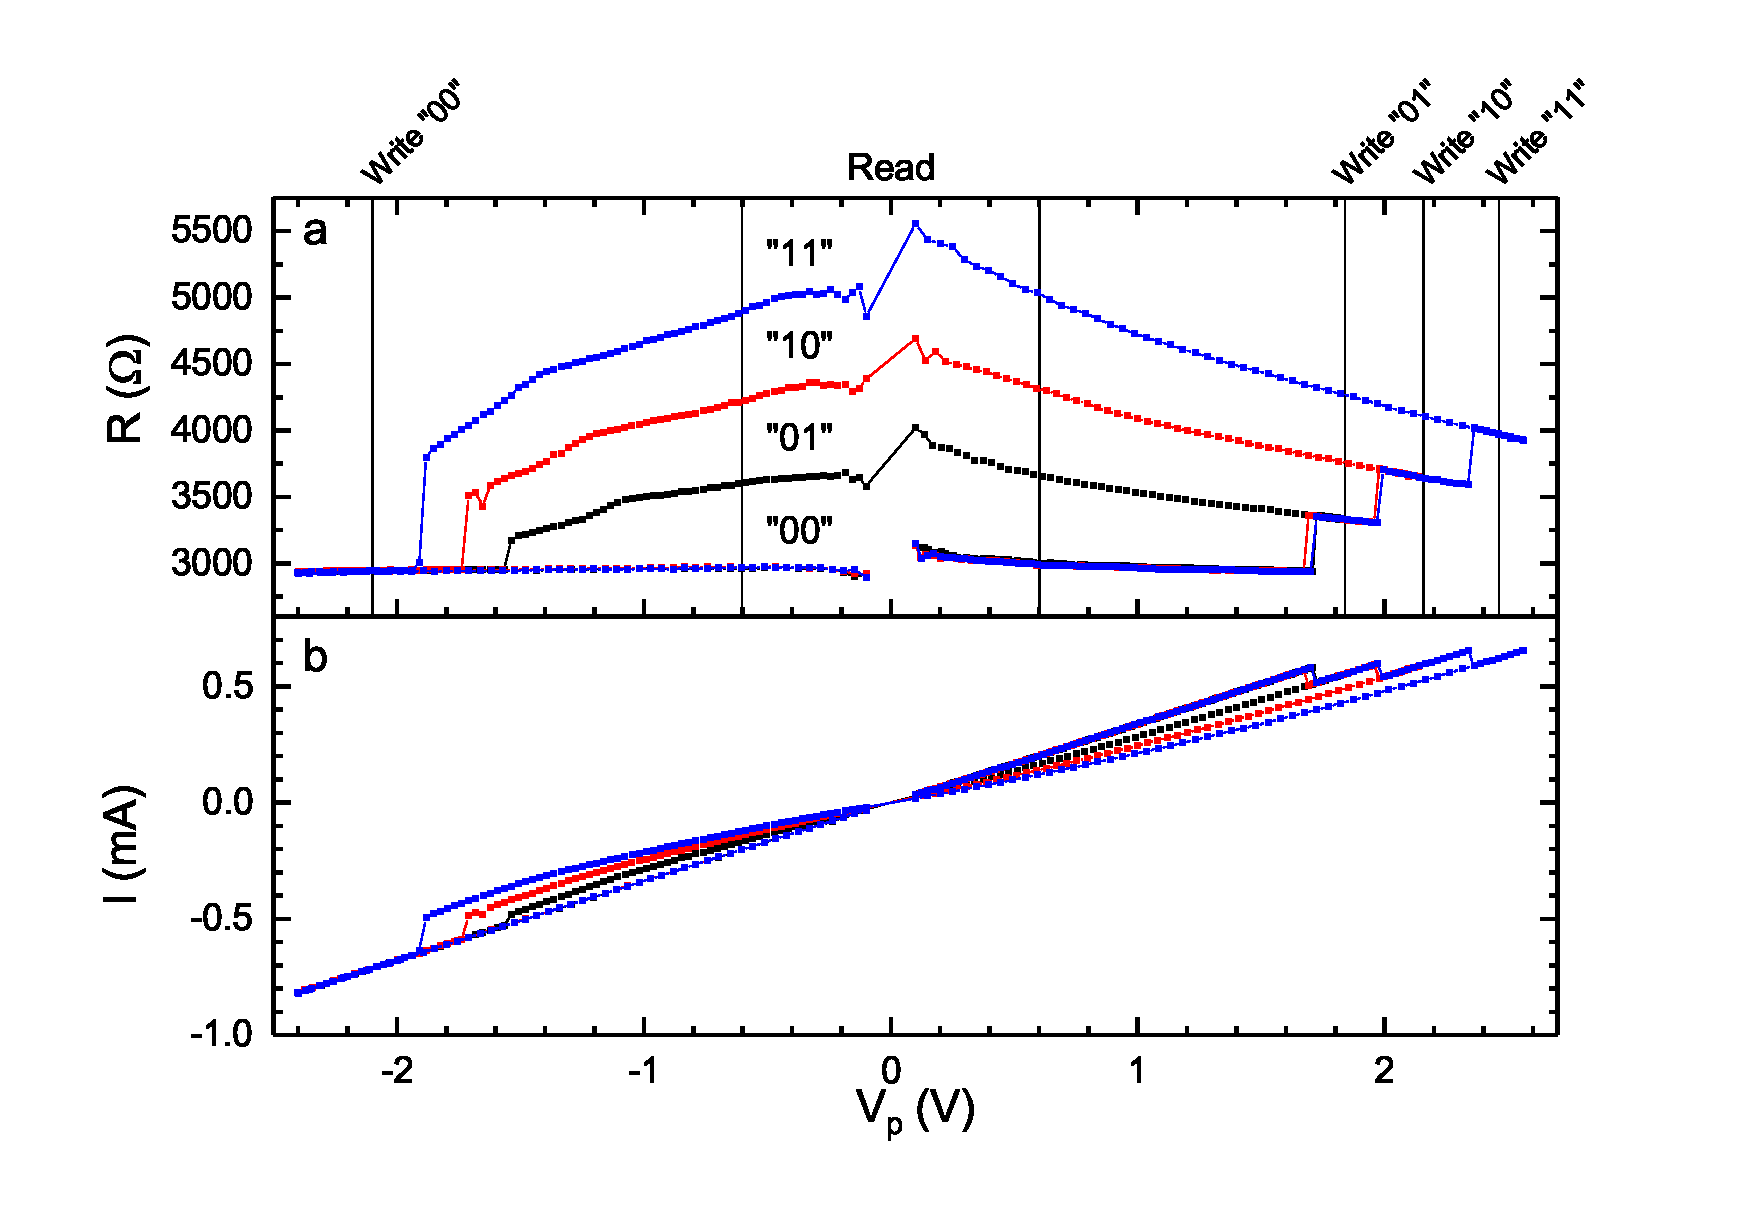
\includegraphics[width=0.5\paperwidth]{img/05/ResultsCIMS2.eps}
        \caption{Rezultaty pomiaru CIMS dla 2-bitowej struktury pamiętającej. Zaproponowano kodowanie binarne, napięcia do zapisu i region bezpieczny dla odczytu (a). Zmiany prądu w czasie pomiarów (b).}
        \label{ExperimentMeasurementCIMS2}
    \end{figure}

    \begin{figure}[H]
        \centering
        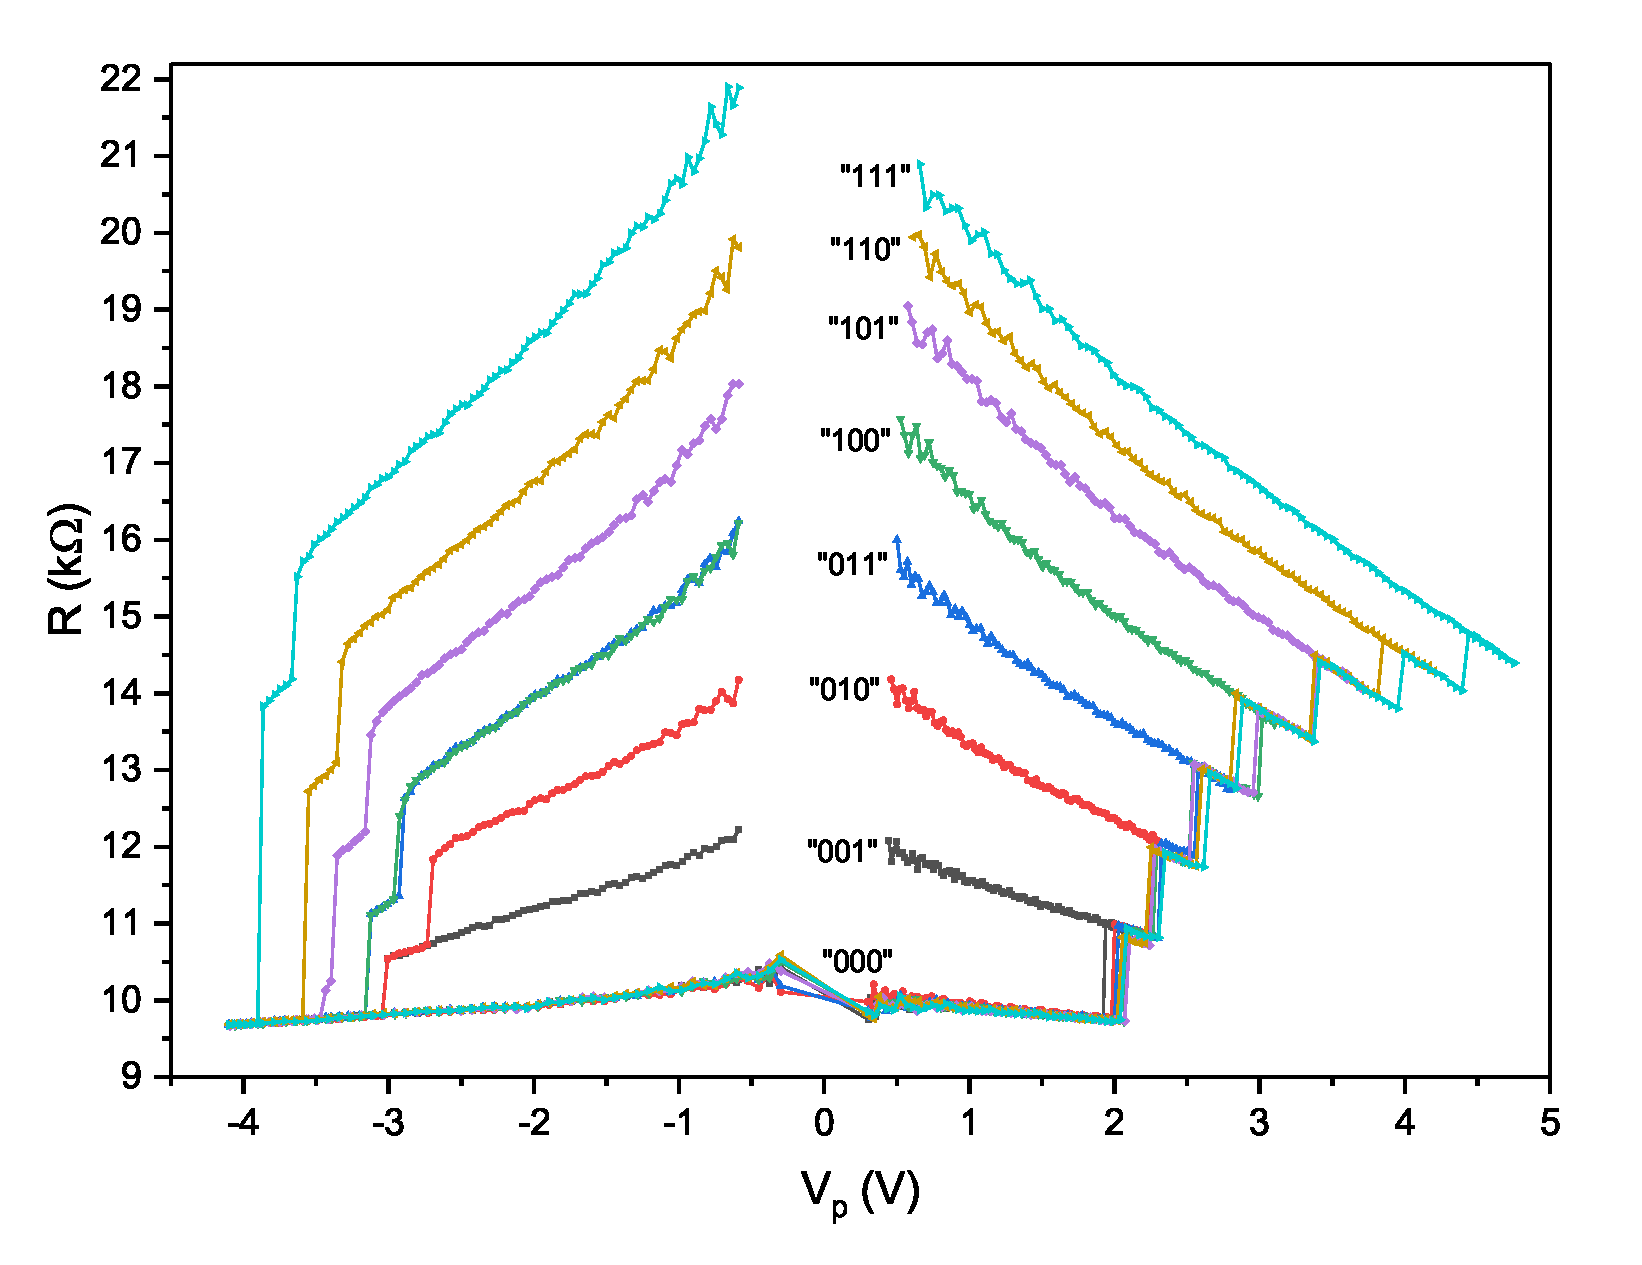
\includegraphics[width=0.5\paperwidth]{img/05/ResultsCIMS3.eps}
        \caption{Rezultaty pomiaru CIMS dla 3-bitowej struktury pamiętającej. Zaproponowano kodowanie binarne.}
        \label{ExperimentMeasurementCIMS3}
    \end{figure}

    
    W podsumowaniu omówiono wszystkie osiągnięte rezultaty a także zwrócono uwagę na niedoskonałości proponowanego rozwiązania i zaproponowano dalszy kierunek badan i optymalizacji.